\chapter[Electron Density Mapping in Carina Nebula]{Electron Density Mapping in Carina Nebula}
\label{ch:carina}
This chapter presents the methodology and results of mapping the electron density in the Carina Nebula using observations from the Stratospheric Observatory for Infrared Astronomy (SOFIA) and the Deep Space Network (DSN).
Carina is a major target for ASTHROS and understanding how to map electron density is one of the key science goals of the mission.
In order to better estimate ASTHROS's capabilities, we embarked on this project to use new observations from SOFIA, which has the same 2.5 meter telescope as ASTHROS, to map the electron density in Carina Nebula.
This can give us a clearer estimate of the sensitivity necessary to map [NII] 205 and 122 $\mu$m lines when ASTHROS is in flight. 

\section{Abstract}
The Carina Nebula is one of the most massive and active star-forming regions in the Milky Way, located approximately 2.3 kpc away in the Carina-Sagittarius arm of the galaxy.
In this work, we present a method to map the electron density in the Carina Nebula using observations of the [NII] 205 $\mu$m fine-structure line and hydrogen radio recombination lines (RRLs) from the Stratospheric Observatory for Infrared Astronomy (SOFIA) and the Deep Space Network (DSN).
We utilize a method used in \cite{pineda2019electron} to calculate the electron density from the ratio of the [NII] 205 $\mu$m line intensity to the RRL intensity.
Additionally, we estimate the [NII] 122 $\mu$m line intensity using the relationship between the two [NII] lines.
These observations show two spectrally distinct regions, the higher density region near the Keyhole Nebula and a lower density region behind the Keyhole Nebula, which we refer to as Carina Extedned.
In the Keyhole Nebula, we find average electron densities of 350 cm$^{-3}$, while in the Carina Extended region, we find average electron densities of 176 cm$^{-3}$.
We compared our results with previous observations from the South Pole Imaging Fabry-Perot Interferometer (SPIFI) and the Infrared Satellite Observatory (ISO) and found that our results are higher than previous measurements.
\section{Keywords}
\keywords{Carina Nebula, Electron Density, [NII] 205 $\mu$m, Hydrogen Radio Recombination Lines, SOFIA, Deep Space Network, ASTHROS}

\section{Introduction}
The Carina Nebula, also known as NGC 3372, is one of the most massive and active star-forming regions in the Milky Way, located approximately $R_{gal}$ = 2.3 kpc away in the Carina-Sagittarius arm of the galaxy \parencite{smith2006census}.
Within Carina is the Keyhole Nebula, located near the center of Carina next to massive stars, such as $\eta$ Carina, which constnatly blasts the nebula with ionizing radiation and stellar winds \parencite{brooks2005simba}.
The nebula's complex structure, which includes dense molecular clouds, ionized gas regions, and young stellar clusters, makes it an ideal laboratory for studying the processes of star formation and feedback from massive stars \parencite{smith2007census}.

Understanding the electron density in star-forming regions like the Carina Nebula is crucial for several reasons. 
Firstly, the electron density can be used as a diagnostic tool for the pressure and density of the ionized gas within star forming regions, which can help us understand the conditions under which stars form \parencite{kaasinen2016cosmos}.
At different evolutionary stages, the electron density in an HII region like Carina can vary significantly, providing insights into the physical processes at play in these regions \parencite{goldsmith2024electron}.
Additionally, understanding the relationship between electron density at low redshift regions like Carina and help inform our understanding of the electron density in high redshift galaxies, which can be used to study the evolution of galaxies and the interstellar medium (ISM) over cosmic time \parencite{shirazi2014stars}.

In this work, we aim to map the electron density in the Carina Nebula using observations of the [NII] 205 $\mu$m fine-structure line and hydrogen radio recombination lines (RRLs). 
These lines are sensitive to the conditions of ionized gas and provide complementary information about the nebula's physical properties. 
We utilize a method used in \cite{pineda2019electron} to calculate the electron density from the ratio of the [NII] 205 $\mu$m integrated intensity to the RRL integrated intensity.
\section{Observations}
Our observations come from two main sources, SOFIA and the DSN.
In addition to these data sources, we also use ancillary data from the South Pole Imaging Fabry-Perot Interferometer (SPIFI) and the Infrared Satellite Observatory (ISO) to compare our results \parencite{oberst2011205}.
Additonally, we utilize the Atacama Large Millimeter/submillemeter Array (ALMA) for continuum brightness temperature observations in our calculations \parencite{Rebolledo_2021}.

\subsection{SOFIA --- Stratospheric Observatory for Infrared Astronomy}
SOFIA was a joint project of NASA and the German Aerospace Center (DLR), operating from a Boeing 747 aircraft equipped with a 2.5-meter telescope designed for infrared observations.
On SOFIA was the German REceiver for Astronomy at Terahertz frequencies (GREAT) which observed a wide range of spectral lines between 1.25 and 2.5 THz using a heterodyne receiver \parencite{heyminck2012great}.
Using the L1 channel of GREAT, we observed the [NII] 205 $\mu$m line in the Carina Nebula, providing a high-resolution spectral cube of the region.
This spectral cube was generated using the SOFIA Data Processing System (DPS) which processes raw data from the instruments, calibrates it, and combines multiple exposures to create a final spectral cube \parencite{shuping2014overview}.
The cube itself is a 36 by 36 pixel map spanning \qty{11}{\arcminute} by \qty{11}{\arcminute} with a 202 spectral channels covering a velocity range of -110 to 90 km/s with a velocity resolution of 1 km/s.
The data has a beam size of \qty{20.77}{\arcminute}  and is tuned to a frequency of 1.45 MHz for measuring the [NII] 205 $\mu$m line.
Due to the calibration, the values are already in Main Beam Brightness Temperature (K$_{mb}$) units.

\subsection{DSN --- Deep Space Network}
The DSN is a global network of antennas that supports interplanetary spacecraft missions and radio astronomy observations.
For radio astronomy, the DSN Deep Space Station 43 (DSS-43) in Canberra, Australia, is equipped with a 70-meter dish that can observe radio recombination lines (RRLs) at frequencies within the K-band (17 to 27 GHz) \parencite{virkler2020broadband}.
Our RRL data for Carina Nebula was collected using the DSS-43 antenna as an average of the RRL observations from H70$\alpha$ (18.768 GHz) to H62$\alpha$ (26.939 GHz).
This average was taken by scaling all the components to the central value of H67$\alpha$ (21.385 GHz) and gridding the data to match the lowest frequency, H70$\alpha$.
The resultant map is much larger than the original SOFIA map, spanning \qty{150}{\arcminute} by \qty{76}{\arcminute} (343 x 335 pixels) with a beam size of \qty{56}{\arcsecond} and a spectral resolution of 2.4 km/s across 165 channels (-300 to 98 km/s).
Unlike the SOFIA data, the RRL data is in units of antenna temperature (K$_{Ta*}$), which is the raw output of the radio telescope before calibration.
Using the efficiency of the antenna (0.5 for DSS-43), the data will need to be converted to the Main Beam Brightness Temperature (K$_{mb}$) units for comparison with the SOFIA data.

\subsection{ALMA --- Atacama Large Millimeter/submillimeter Array}
Our radio continuum brightness temperature data comes from the ALMA observations of the Carina Nebula.
ALMA is an array of radio telescopes located in the Atacama Desert in Chile, designed to observe the universe at millimeter and submillimeter wavelengths.
We utilize data from \cite{Rebolledo_2021}, which provides a continuum brightness temperature map of the Carina Nebula between 1-3 GHz with a beam of \qty{24}{\arcsecond} spanning \qty{613}{\arcminute} by \qty{297}{\arcminute} (3574 x 3415 pixels).
This data is in units of Jy/beam, which is a common unit for radio continuum observations but needs to be converted to brightness temperature (K) for our calculations.

\subsection{Other Ancillary Data}
\cite{oberst2011205} provides line intensities for ISO's [NII] 122 $\mu$m line and SPIFI's [NII] 205 $\mu$m line in the form of tables with coordinates and integrated intensities.
These values need to be processed into data cubes to be useful in our analysis.
When using FITS data, a World Coordinate System (WCS) is used to map the pixel coordinates to celestial coordinates, allowing for easy comparison of data from different instruments.
Without this WCS information, we cannot directly compare the data cubes.
Using the provided coordinates in the tables, we can estimate a WCS for both of these datasets as explained in Section \ref{carina/sec:fits_fit}.
Additionally, the data is in units of line intensity (W m$^{-2}$ sr$^{-1}$) which needs to be converted to Main Beam Brightness Temperature (K$_{mb}$) for comparison with the SOFIA data.
Between ISO and SPIFI, there are only about 3 pixels that overlap with the SOFIA data, so we will not be using these datasets in our analysis but will be using them to compare our results.

\begin{figure}
    \centering
    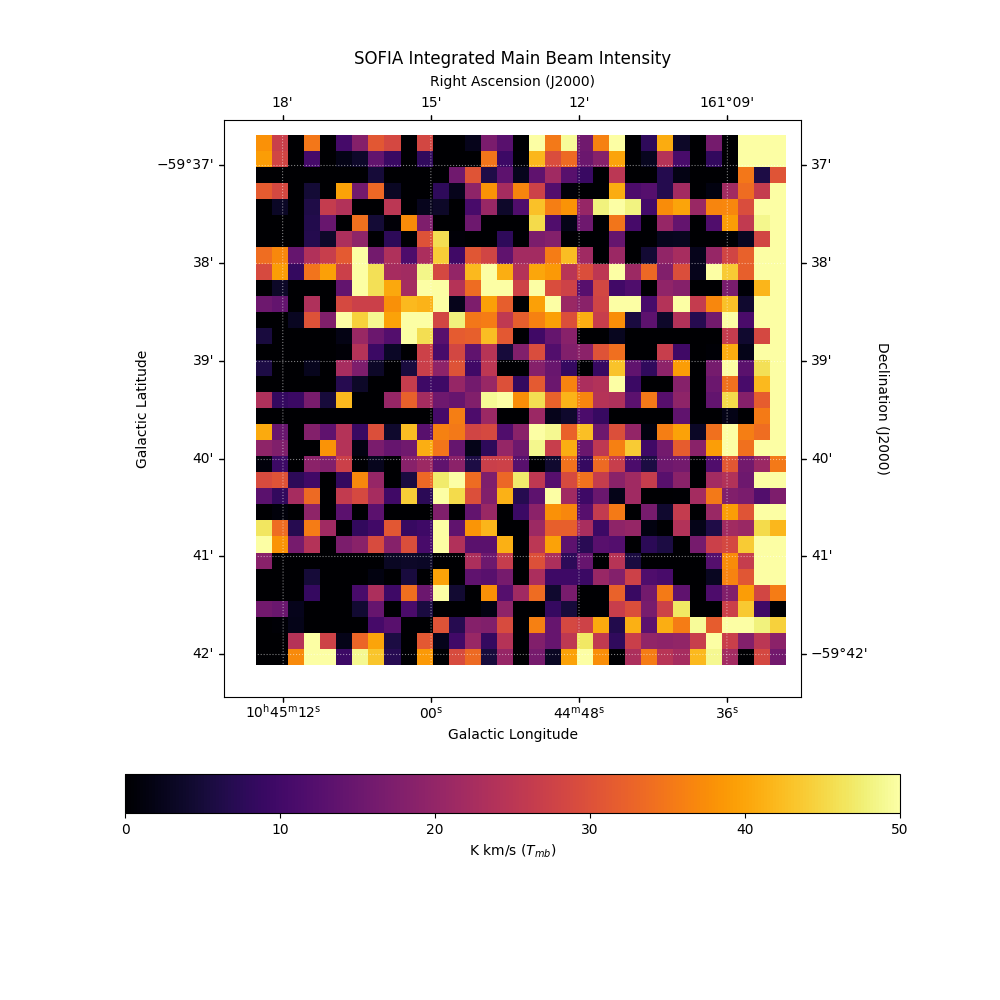
\includegraphics[width=0.6\textwidth]{figs/carina/raw_NII.png}
    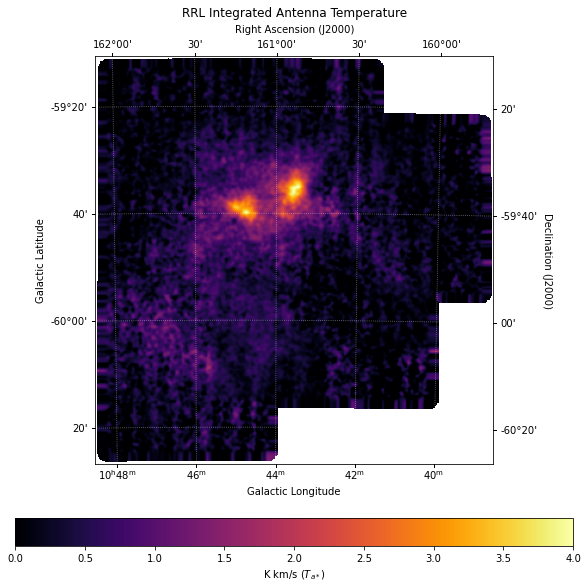
\includegraphics[width=0.6\textwidth]{figs/carina/raw_RRL.png}
    \caption[Raw Data Cubes for {[}NII{]} and RRLs in Carina Nebula]{
        The raw data cubes for the [NII] 205 $\mu$m line (top) and the RRL data (bottom). 
        Both lines are integrated intensities across the entire spectral range of the dataset.
        The [NII] 205 $\mu$m line is shown using Main Beam Temperatures, while the RRL data is shown in Antenna Temperature.
        }
    \label{carina/fig:raw_data}
\end{figure}

\section{Methodology}
Our analysis follows the methodology outlined in \cite{pineda2019electron}, which describes how to calculate electron density from the ratio of [NII] 205 $\mu$m line intensity to the intensity of Hydrogen Radio Recombination Lines (RRLs).
This analysis was done using the \texttt{spectral-cube} package in Python, which allows for efficient manipulation of spectral data cubes \parencite{robitaille2016spectral}.
\texttt{spectral-cube} wraps many of the functionalities of the \texttt{astropy} package, which is a core package for astronomy in Python \parencite{astropy:2013, astropy:2018, astropy:2022}.
Our methodology for analysis consists of preprocessing the data cubes to ensure they are on the same grid with the same spatial and spectral resolutions, convolving the [NII] 205 $\mu$m data with the beam of the RRL data, and then performing calculations to derive the electron density from the ratio of the two lines.
In addition to the electron density, we are also able to estimate the [NII] 122 $\mu$m line intensity, which whose ratio with the [NII] 205 $\mu$m line can be used to estimate electron density as well \parencite{goldsmith2015herschel}.
Figure \ref{carina/fig:raw_data} shows the raw data cubes for both the [NII] 205 $\mu$m line and the RRL data.

\subsection{Pre-processing the Data Cubes}
In order to properly compare the two data cubes, we first need to pre-process everything to ensure our data points match both spatially and spectrally.
First, we need our data to be in the same units, so we will convert the RRL data from antenna temperature (K$_{Ta*}$) to Main Beam Brightness Temperature (K$_{mb}$) using the efficiency of the antenna as shown in Equation \ref{eq:mb_temp}, where $T_{Ta*}$ is the antenna temperature and $\eta_{mb}$ is the main beam efficiency of the antenna.
\begin{equation}
    T_{mb} = \frac{T_{Ta*}}{\eta_{mb}}
    \label{eq:mb_temp}
\end{equation}
Next we need to ensure both datasets have a common beam size.
As the SOFIA data has a smaller beam than the RRL data, we will convolve the [NII] 205 $\mu$m data with a Gaussian kernel that matches the beam size of the RRL data.
This is handled by the \texttt{spectral-cube} package, which uses the \texttt{astropy.convolution} module to convolve the data with a Gaussian kernel that matches the beam size of the RRL data.
We perform this step first to ensure that the [NII] 205 $\mu$m data is properly smoothed to match the RRL data before interpolating the data to a common grid, where we may lose some spatial resolution. 

Following this, we spectrally interpolate the [NII] 205 $\mu$m data to match the larger spectral resolution of the RRL data.
We also crop both data cubes to the same spectral range. 
This is accomplished by convolving the [NII] 205 $\mu$m data with a Gaussian kernel with a standard deviation with that matches the difference in spectral resolution between the two datasets as shown in Equation \ref{eq:gaussian_kernel}, where $\sigma$ is the standard deviation of the Gaussian kernel, $\Delta \nu_{[NII]}$ is the spectral resolution of the [NII] 205 $\mu$m data, and $\Delta \nu_{RRL}$ is the spectral resolution of the RRL data.
\begin{equation}
    \sigma_{FWHM} = \frac{\Delta \nu_{RRL}^2 - \Delta \nu_{[NII]}^2}{\sqrt{8\ln(2)}}
    \label{eq:gaussian_kernel}
\end{equation}
After spectral interpolation, both spectral cubes are sent through a Savitzky-Golay filter to smooth the data and improve our signal-to-noise ratio (SNR). 
We use a polynomial order of 3 and a window length of 10 spectral channels, which is sufficient to smooth the data without losing too much spectral resolution. 
This process is outlined by \cite{pineda2019electron} and is implemented using the \texttt{savgol\_filter} function from \texttt{scipy} \parencite{2020SciPy-NMeth}.
Figure \ref{carina/fig:spectral_means} shows the mean spectra of both the [NII] 205 $\mu$m line and the RRL data at each step of spectral interpolation and smoothing.

\begin{figure}
    \centering
    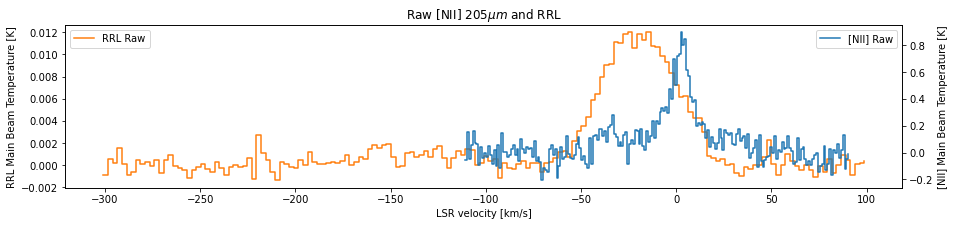
\includegraphics[width=0.95\textwidth]{figs/carina/spec_raw.png}
    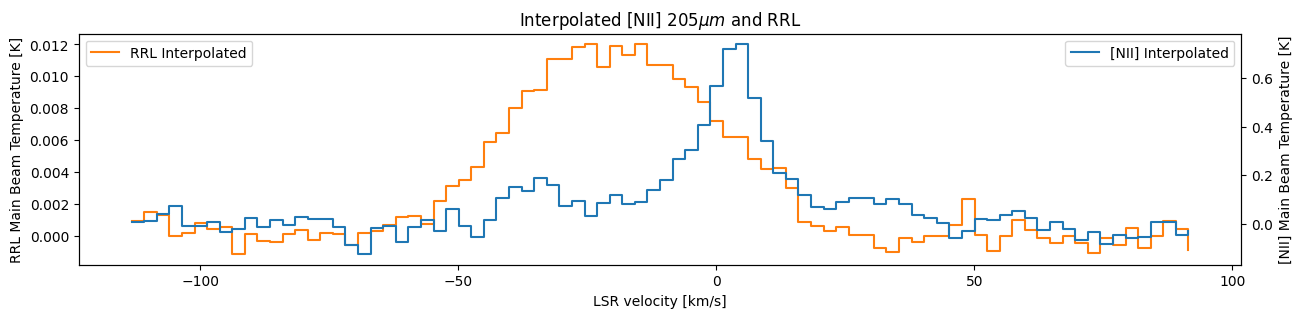
\includegraphics[width=0.95\textwidth]{figs/carina/spec_inter.png}
    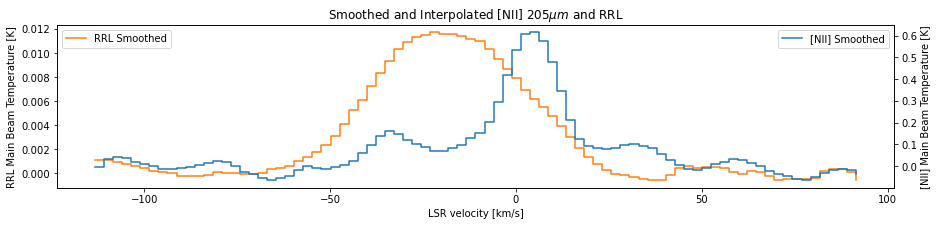
\includegraphics[width=0.95\textwidth]{figs/carina/spec_smooth.png}    
    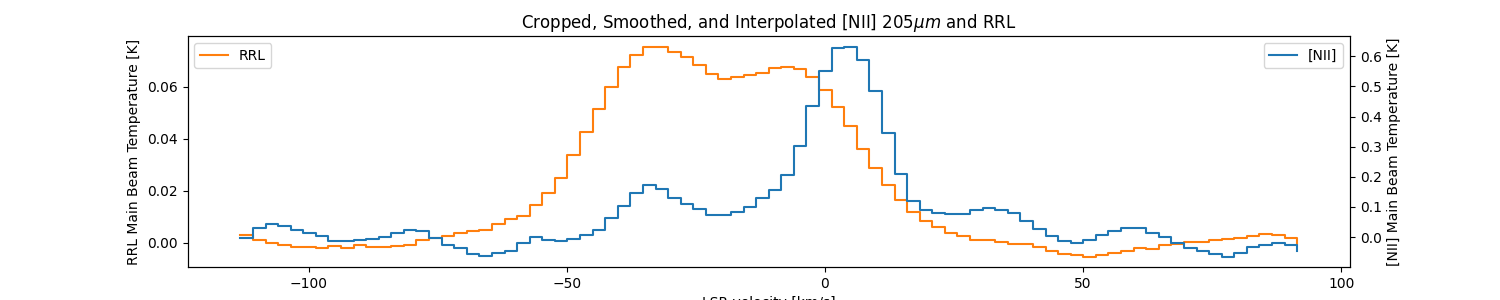
\includegraphics[width=0.95\textwidth]{figs/carina/spec_final.png}
    \caption[Mean Spectra of {[}NII{]} 205 $\mu$m and RRL Data During Preprocessing]{
        The mean spectra of the [NII] 205 $\mu$m line (blue) and the RRL line (orange) at each step of preprocessing.
        Note that the first three panels show the mean spectra of the entire RRL region which includes more area than the SOFIA data.
        The top panel shows the raw spectra prior to any spectral interpolation or smoothing.
        The second panel shows the spectra after spectral interpolation to the RRL data's spectral resolution and cropping to the same common range.
        The third panel shows the spectra after applying a Savitzky-Golay filter to smooth the data.
        The final panel shows the final spectra after spatial cropping and interpolation.
        }
    \label{carina/fig:spectral_means}
\end{figure}

After the spectral interpolation and smoothing, we can crop both data cubes to the same spatial region and reproject them to a common grid.
The RRL map covers a much larger area than the SOFIA map, so we will need to crop the RRL data.
Using the world extrema of the SOFIA data, we can create a subcube of the RRL data whose bounds match the SOFIA data.
The spatial resolution of the SOFIA data is smaller than the RRL data, so we use the \texttt{reproject} function from \texttt{spectral-cube} to interpolate the SOFIA data to the RRL data's grid.
This matches the WCS of both data cubes, allowing us to compare the two datasets directly.
After this step, we have two data cubes that are on the same grid, with the [NII] 205 $\mu$m data convolved to match the beam size of the RRL data and both datasets having the same spatial and spectral resolution as shown in Figure \ref{carina/fig:processed_data}.

\begin{figure}
    \centering
    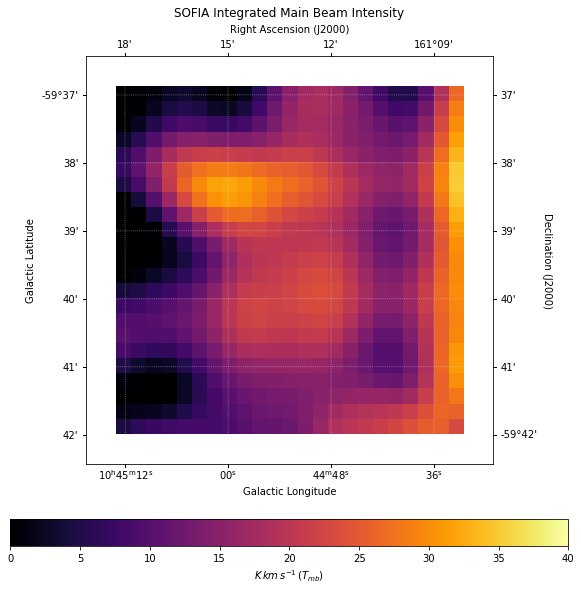
\includegraphics[width=0.6\textwidth]{figs/carina/final_NII.png}
    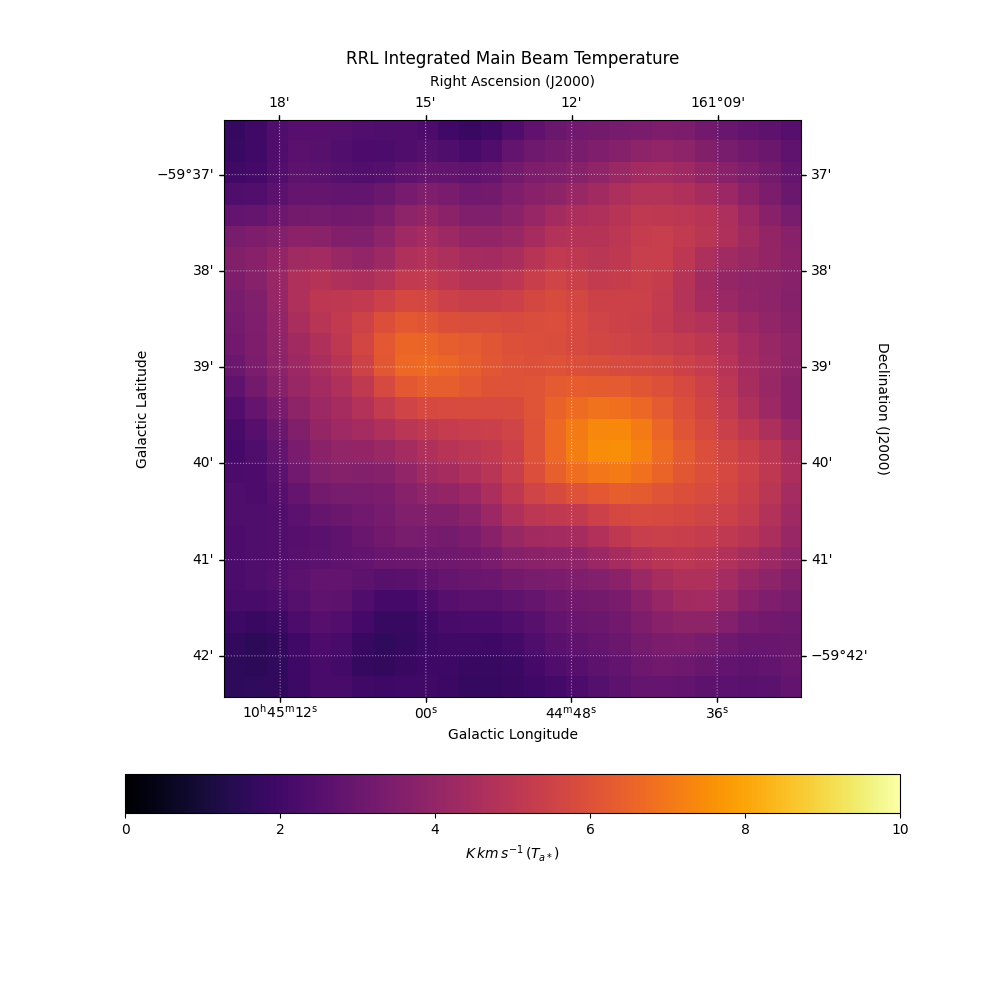
\includegraphics[width=0.6\textwidth]{figs/carina/final_RRL.png}
    \caption[Preprocessed Data Cubes for {[}NII{]} and RRLs in Carina Nebula]{
        The processed data cubes for the [NII] 205 $\mu$m line (top) and the RRL data (bottom).
        Both lines are the integrated main beam intensities across the entire spectral range of the dataset.
        }
    \label{carina/fig:processed_data}
\end{figure}

In addition to the above preprocessing steps, we also need to perform some additional steps to prepare the ALMA continuum brightness temperature data.
First, we need to convert the ALMA data from Jy/beam to K to get our brightness temperature.
This is done using Equation \ref{carina/eq:alma_temp}, where $T_b$ is the brightness temperature in K, $S$ is the flux density in Jy/beam, $\lambda$ is the wavelength in centimeters, and $\theta$ is the beam size in arcminutes \parencite{rohlfs2013tools}.
\begin{equation}
    T_C = \frac{S\ \lambda^2}{2.65\ \theta^2}
    \label{carina/eq:alma_temp}
\end{equation}
The also needs to be corrected to match the frequency of the RRL data.
This is accomplished by using a power law to scale the brightness temperature to the frequency of the RRL data as shown in Equation \ref{carina/eq:alma_freq}, where $T_{Bf}$ is the final brightness temperature in K, $T_{Bi}$ is the initial brightness temperature in K, $\nu_{f}$ is the final frequency in GHz, $\nu_i$ is the initial frequency in GHz, and $\alpha$ is the spectral index.
\begin{equation}
    T_{Bf} = T_{Bi} \left( \frac{\nu_f}{\nu_i} \right)^\alpha
    \label{carina/eq:alma_freq}
\end{equation}
For Carina Nebula, we use a spectral index of -0.1, which is used for optically thin thermal bremsstrahlung emission \parencite{salatino2012spectral}.
As our RRL data is scaled to the H67$\alpha$ line, we will use the frequency of this line (21.385 GHz) as our final frequency, extrapolating from the ALMA data which is centered around 2.1 GHz.
Finally, while ALMA data is not a spectral cube, \texttt{spectral-cube} can handle spatial interpolation of 2D data as well.
We use the WCS of the final [NII] 205 $\mu$m data cube to reproject the ALMA data to the same grid.

\subsection{Calculating Electron Density}
The first step to calculating electron density is to see how the [NII] 205 $\mu$m line intensity and the RRL intensity are related.
We begin with the following equation for the integrated intensity of the [NII] line \parencite{pineda2019electron}:
\begin{equation}
    \label{carina/eq:intensity_NII}
    \int{T_{mb}^{[NII]}} d\nu = \frac{A_{ul}hc^3N_u}{8\pi k_b \nu_{ul}^2}\\
\end{equation}
In this equation, $A_{ul}$ is the Einstein A coefficient for spontaneous decay rate, $h$ is Planck's constant, $c$ is the speed of light, $N_u$ is the column density of the upper level, $k_b$ is Boltzmann's constant, and $\nu_{ul}$ is the frequency of the transition.
We can simply this further by noting that the upper level column density, $N_u$, is related to the fractional population of the upper level, $f(^uP_l)$, and the total column density of ionized nitrogen, $N(N^+)$, as follows:
\begin{equation}
    N_u = f(^3P_u) N(N^+)
    \label{carina/eq:N_u}
\end{equation}
There are two fine structure transitions for [NII] at 122 $\mu$m ($^3P_2$ - $^3P_1$) and 205 $\mu$m ($^3P_1$ - $^3P_0$).
Combining Equations \ref{carina/eq:N_u} with \ref{carina/eq:intensity_NII} results in the following equation for the integrated intensity of the [NII] 205 $\mu$m line:
\begin{align}
    \int{T_{mb}^{[NII]}} d\nu &= \frac{A_{ul}hc^3f(^3P_u)N(N^+)}{8\pi k_b \nu_{ul}^2} \\
    &= \num{5.145e14}\ A_{ul}\nu_{ul}^{-2}f(^3P_u)N(N^+)\ [\text{K km/s}]
    \label{carina/eq:intensity_NII_final}
\end{align}
In the simplified version, $A_{ul}$ is in s$^{-1}$, $f(^3P_u)$ is dimensionless, $N(N^+)$ is in cm$^{-2}$, and $\nu_{ul}$ is in Hz.
We utilize PyNeb, a Python package for calculating emission line intensities, to obtain our Einstein A coefficient, $A_{ul}$ and the fractional population of the upper level, $f(^3P_u)$ \parencite{luridiana2015pyneb, froese2004breit,7288EL, tayal2011electron}.


Now we can look at the integrated intensity of the RRL line using the following equation \parencite{pineda2019electron}:
\begin{equation}
    \int{T_{mb}^{RRL}} d\nu = \num{1.87e-7}\ \frac{n_e N(H^+)}{\nu_{RRL} T_e^{3/2}}\ [\text{K km/s}]
    \label{carina/eq:intensity_RRL}
\end{equation}
For the RRL, $n_e$ is the electron density in cm$^{-3}$, $N(H^+)$ is the column density of ionized hydrogen in cm$^{-2}$, $\nu_{RRL}$ is the frequency of the RRL in Hz, and $T_e$ is the electron temperature in K.
Because the hydrogen recombination lines can be affected by non-local thermal equilibrium (NLTE) effects, we also need to account for the deviation from LTE in the RRL emission \parencite{gordon2002radio}.
\begin{equation}
    G_{NLTE}(n_e,T_C) = \frac{T^{RRL}}{T^{RRL}_{NLTE}} = b_n \left[1-\frac{1}{2}\tau_c \beta_n\right]
    \label{carina/eq:G_NLTE}
\end{equation}
In this equation, $b_n$ and $\beta_n$ are the departure coefficient and amplification factor for a specific principal quantum number $n$, and $\tau_c$ is the continuum opacity. 
$\tau_c$ can be calculated using the continuum brightness temperature, $T_C$, and the electron temperature , $T_e$, as follows \parencite{goldsmith2024electron}:
\begin{equation}
    \tau_c = \frac{T_C}{T_e}
    \label{carina/eq:tau_C}
\end{equation}
The GNLTE coefficients are obtained using a Fortran program in the appendix of \cite{gordon2002radio}, which was later wrapped in Python by \cite{2017ascl.soft07001W}.
These values depend on electron density, $n_e$, and electron temperature, $T_e$, for a given principal quantum number $n$.
A precomputed table of these values is used to interpolate the values for our specific electron density at $T_e$ = 8000 K.
Adding on this factor, we can rewrite Equation \ref{carina/eq:intensity_RRL} line as follows:
\begin{equation}
    \int{T_{mb}^{RRL}} d\nu = \num{1.87e-7}\ \frac{N(H^+)}{\nu_{RRL} T_e^{3/2}}\ n_e\ G_{NLTE}(n_e, T_c)\ [\text{K km/s}]
    \label{carina/eq:intensity_RRL_final}
\end{equation}

Finally, we can compute the ratio of Equation \ref{carina/eq:intensity_NII_final} and \ref{carina/eq:intensity_RRL_final} to get the following equation:
\begin{equation}
    R^{[NII]}_{RRL} = \frac{\int{T^{[NII]}_{mb} d\nu}}{\int{T^{RRL}_{mb} d\nu}} = \num{2.75e21}\ \frac{A_{ul}\nu_{RRL}T_e^{3/2}}{\nu_{ul}^2}\ \frac{N(N^+)}{N(H^+)}\ \frac{f(^3P_u)}{n_e G_{NLTE}(n_e,T_c)}
    \label{carina/eq:ratio_final}
\end{equation}
Most of the terms in this equation are constants that do not depend on the electron density, $n_e$, except for the last term, RHS = $f(^3P_u)/n_e G_{NLTE}(n_e,T_c)$.
The remaining unknown terms $T_e$ the electron temperature in K, and $N(N^+)/N(H^+)$, the abundance ratio of ionized nitrogen with respect to ionized hydrogen, can be estimated using the distance to the Galactic center, $R_{gal}$, in kpc \parencite{pineda2019electron, balser2015azimuthal, esteban2018revisiting}:
\begin{align}
    T_e &= (4446 \pm 301) + (467 \pm 34) R_{gal} \\
    12 + \log(N/H) &= (8.21 \pm 0.09) - (0.059 \pm 0.009) R_{gal}
\end{align}

Rearranging Equation \ref{carina/eq:ratio_final} to isolate the term that depends on electron density allows us to look at the relationship between those terms and electron density in Figure \ref{carina/fig:gnlte_curves}.
The curves are generated using fractional population data from \cite{luridiana2015pyneb} and GNLTE coefficients from \cite{gordon2002radio} to write a function that calculates RHS for a given electron density, $n_e$, and continuum brightness temperature, $T_c$.
Because these curves are related to the ratio of the [NII] 205 $\mu$m line intensity to the RRL intensity, we can use them to calculate the electron density for a given ratio of intensities.
This is accomplished by calculating the ratio of the integrated intensities and dividing by the constant terms. 
Then we can use a root solving algorithm, such as \texttt{scipy.optimize.fsolve}, find the value of electron density that whose RHS matches the calculated ratio \parencite{2020SciPy-NMeth}.
This process is repeated for each pixel in the [NII] 205 $\mu$m data cube, resulting in a map of electron density across the Carina Nebula.

\begin{figure}
    \centering
    \begin{subfigure}[t]{0.45\textwidth}
        \centering
        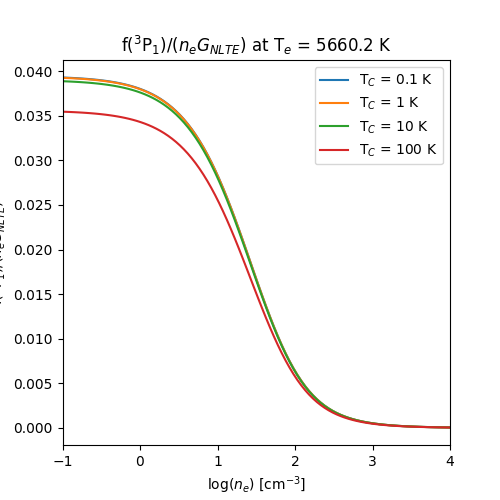
\includegraphics[width=\textwidth]{figs/carina/gnlte_curves.png}
        \caption{
        The fractional population of the 205 $\mu$m level of ionized nitrogen, $f(^3P_1)$, and the GNLTE coefficients, $G_{NLTE}(n_e,T_c)$, as a function of electron density for various continuum brightness temperatures.
        }
        \label{carina/fig:gnlte_curves}
    \end{subfigure}%
    ~
    \begin{subfigure}[t]{0.45\textwidth}
        \centering
        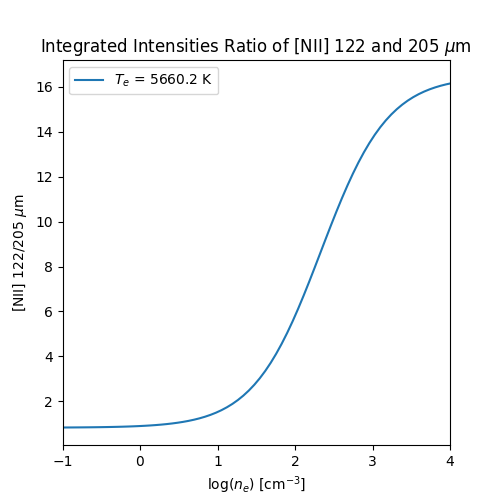
\includegraphics[width=\textwidth]{figs/carina/nii_curves.png}
        \caption{Ratio of the integrated intensities of the two lines of [NII] as a function of electron density at an electron temperature of 5662 K.}
        \label{carina/fig:nii_curves}
    \end{subfigure}
    \caption{Ratios of Electron Density with Fractional Population and G$_{NLTE}$ Coefficients for Calculating Electron Density and [NII] 122 $\mu$m}
\end{figure}

In addition to electron density, we can also estimate the [NII] 122 $\mu$m line intensity using the relationship between the two [NII] lines \parencite{goldsmith2015herschel}.
The [NII] 205 $\mu$m and 122 $\mu$m lines correspond with the $^3P_2$ - $^3P_1$ and $^3P_1$ - $^3P_0$ transitions, respectively. 
We can take the ratio of these two lines to see their dependency on electron density by using Equation \ref{carina/eq:intensity_NII_final}:
\begin{equation}
    \frac{\int{T_{mb}^{[NII]\ 122}} d\nu}{\int{T_{mb}^{[NII]\ 205}} d\nu} = \frac{A_{21}f(^3P_2)\nu^2_{205}}{A_{10}f(^3P_1)\nu_{122}^2}
    \label{carina/eq:intensity_NII_ratio}
\end{equation}
This ratio relies on electron temperature and density in the form of the fractional populations $f(^3P_1)$ and $f(^3P_2)$.
Figure \ref{carina/fig:nii_curves} shows the ratio of the two lines at the calculated electron temperature for Carina Nebula, which is approximately 5660 $\pm$ 313.7 K.


\subsection{Uncertainties}
The primary sources of uncertainty in our electron density calculations come from the actual measurements of the [NII] 205 $\mu$m line and the RRL data, as well as the usage of $R_{gal}$ to estimate the electron temperature and nitrogen abundance.
As we are taking the integrated intensities of the [NII] 205 $\mu$m line and the RRL data, we can calculate the uncertainties in these measurements using the RMS noise of the data cubes.
We calculate this by taking the standard deviation of the data cube in a region where we expect no signal, such as the edges of the spectral range for each pixel, far away from the center of the spectral line where Carina is located. 
This produces a per channel noise map for each pixel in the data cube which we can use to calculate the uncertainties in our integrated intensities as follows:
\begin{equation}
    \sigma_{int} = \text{RMS} \times \sqrt{N_{chan}} \times \Delta \nu
    \label{carina/eq:uncertainty_intensity}
\end{equation}
This uncertainty, along with the uncertainties in $T_e$ and $N(N^+)/N(H^+)$, can be propagated through the calculations to estimate the uncertainty of the value used to calculate the electron density in the root solving algorithm.

To calculate electron density, we use a Monte Carlo approach, where we randomly sample from a normal distribution centered around the measured value with a standard deviation equal to the uncertainty.
We then solve for the electron density using the sampled values and repeat this process many times (e.g., 1000 iterations) to generate a distribution of electron density values.
This distribution can then be used to calculate the mean and standard deviation of the electron density for each pixel in the map, providing us with an uncertainty estimate for our electron density calculations.
This method was chosen over direct propagation of uncertainties because it allows us to account for the non-linear relationship between the electron density and the ratio of intensities.

\subsection{Aligning SPIFI and ISO Data}
\label{carina/sec:fits_fit}
To align the SPIFI and ISO data with the SOFIA data, we need to create a World Coordinate System (WCS) for each dataset.
Given that we have a table of coordinate points and knowledge that these points are in a grid-like pattern, we can use a bit of image matrix manipulation to create a WCS for each dataset.
A FITS header contains information about a data cube is normally parsed by programs like \texttt{astropy.io.fits} to create a WCS object that can be used to map pixel coordinates to celestial coordinates.
We do not have a FITS header for the SPIFI and ISO data, so we will need to create one ourselves.
The key values we need to set in the FITS header are the following:
\begin{itemize}
    \item \texttt{CRPIX1} and \texttt{CRPIX2}: The reference pixel coordinates in the x and y dimensions, respectively.
    \item \texttt{CRVAL1} and \texttt{CRVAL2}: The celestial coordinates of the reference pixel in degrees.
    \item \texttt{CDELT1} and \texttt{CDELT2}: The pixel size in degrees in the x and y dimensions, respectively.
    \item \texttt{CROTA1} and \texttt{CROTA2}: The rotation angle of the coordinate system in degrees.
\end{itemize}

Our first step is to determine the reference pixel coordinates, which we can set to the center of the data cube.
If our pixels are located on a grid, each pixel will have a both an index and celestial coordinate.
To estimate the index grid, we can use Principal Component Analysis (PCA) to align the coordinates to their principal axes \parencite{wold1987principal}.
In the case of a uniform grid rotated at some angle, this rotates the grid to align with the x and y axes.
At that point, we query a K-Dimensional Tree of these points to find the median spacing between the points.
We can then sort the x and y coordinates and use the following equation to determine each index:
\begin{equation}
    \text{index} = \left\lfloor \frac{\text{coordinate} - \text{min coordinate}}{\text{spacing}} \right\rfloor - \text{min index}
    \label{carina/eq:index}
\end{equation}
This will give us a mapping of each coordinate to its index in the grid.

The PCA step can be skipped if we have a good estimate of the rotation angle of the grid.
In the case of the SPIFI data, this method works well for one half of the data, but not the other half.
In this case, we can use the first half of the data to estimate the rotation angle and then apply that angle to the second half of the data.
Instead of using PCA, we create the rotational matrix using the rotation angle and apply it to the coordinates to align them with the x and y axes 
\begin{equation}
    R_\theta = \begin{bmatrix}
        \cos(\theta) & -\sin(\theta) \\
        \sin(\theta) & \cos(\theta)
    \end{bmatrix}
\end{equation}
where $\theta$ is the rotation angle in radians.

After we have the indices and the world coordinates, we can compute an affine transformation matrix that maps the pixel coordinates to the celestial coordinates.
Using the central index as the reference pixel, we can set the \texttt{CRPIXn} and \texttt{CRVALn} values to its index and coordinates.
We then shift our indices and coordinate points relative to the critical pixel and use these values to calculate the coefficients in our affine transformation matrix.
Our inputs and outputs now look like this:
\begin{align}
    A = \begin{bmatrix}
        \Delta i_1 & \Delta j_1 & 1 \\
        \Delta i_2 & \Delta j_2 & 1 \\
        \vdots & \vdots & \vdots \\
        \Delta i_n & \Delta j_n & 1
    \end{bmatrix}, \quad
    B = \begin{bmatrix}
        \Delta RA_1 & \Delta Dec_1\\
        \Delta RA_2 & \Delta Dec_1\\
        \vdots \\
        \Delta RA_n & \Delta Dec_n
    \end{bmatrix}
\end{align}
where $\Delta i_n$ and $\Delta j_n$ are the pixel coordinates relative to the reference pixel, and $\Delta RA_n$ and $\Delta Dec_n$ are the celestial coordinates relative to the reference pixel.
We can then solve for the coefficients of the affine transformation matrix using the least squares method:
\begin{equation}
    \begin{bmatrix}
        a & b & \_ \\
        c & d & \_
    \end{bmatrix} = A^{-1}B
\end{equation}
This gives us the coefficients for the affine transformation matrix, which we can then use to set the \texttt{CDELTn} values in the FITS header as follows:
\begin{align}
    \texttt{CDELT1} &= \sqrt{a^2 + c^2} \\
    \texttt{CDELT2} &= \sqrt{b^2 + d^2} \\
    \texttt{CROTA1} &= 0 \\
    \texttt{CROTA2} &= \arctan{c/a}
\end{align}

Figure \ref{carina/fig:aligned_fits} shows the aligned SPIFI and ISO data with the SOFIA data.
\begin{figure}
    \centering
    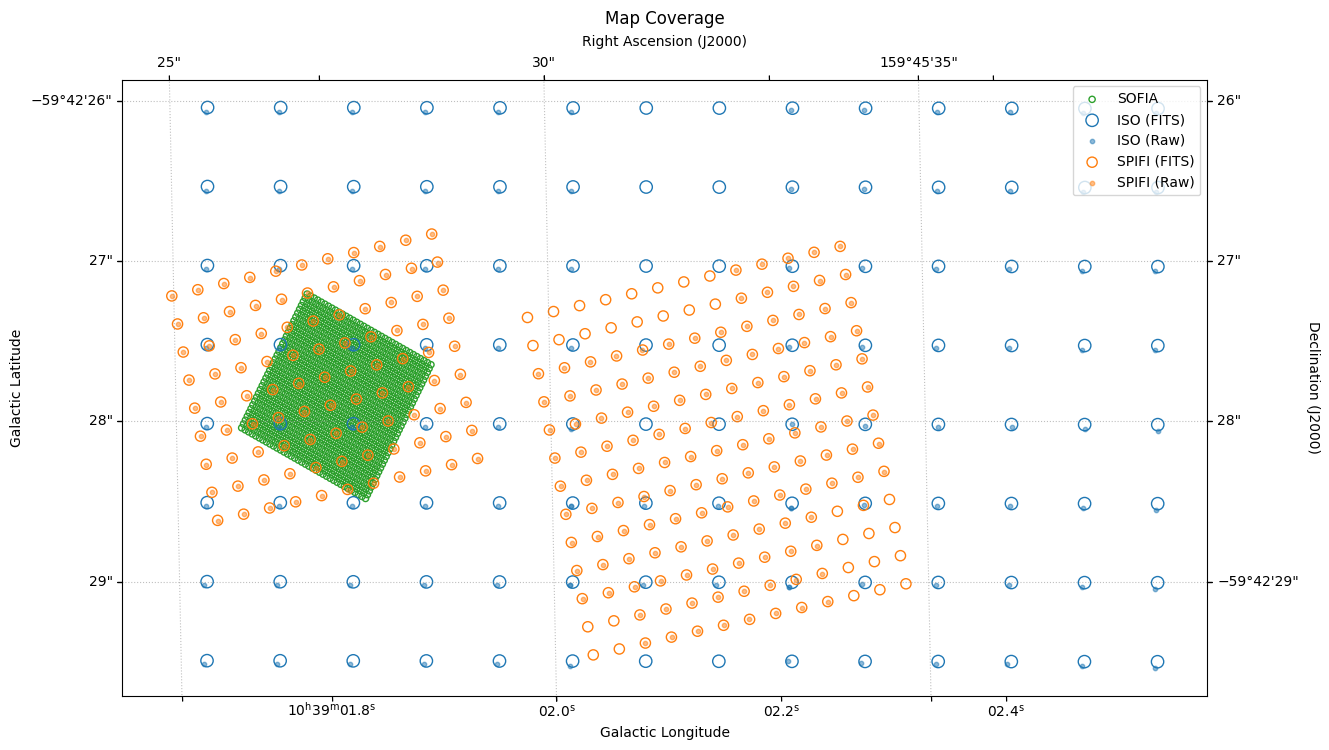
\includegraphics[width=0.9\textwidth]{figs/carina/fits_coverage.png}
    \caption[Aligned SPIFI and ISO Data with SOFIA Data]{
        The aligned SPIFI (top) and ISO (bottom) data with the SOFIA data.
        The SPIFI data is shown in blue, while the ISO data is shown in orange.
        The SOFIA data is shown in green.
        }
    \label{carina/fig:aligned_fits}
\end{figure}

Finally, these values need to be converted from line intensities in W m$^{-2}$ sr$^{-1}$ to integrated main beam intensities in K km/s.
This is accomplished using the following equation \cite{oberst2011205}
\begin{equation}
    \int{T_{mb} d\nu} = \frac{I_\nu \nu^3}{1000 k_b \pi}
\end{equation}

\section{Results}
In observing the spectra of the [NII] 205 $\mu$m line and the RRL data, we can see two distinct regions of interest in the Carina Nebula.
The first region is the Keyhole Nebula which is a prominent feature in the Carina Nebula and is known for its high electron density \cite{brooks2000unlocking}.
Behind the Keyhole Nebula is the Carina Extended region, which is a more diffuse region with lower electron density.
Table \ref{carina/tab:slabs} shows the spectral slabs used to calculate the electron density for both regions.

\begin{table}
    \centering
    \begin{tabular}{|c|c|c|}
        \hline
        Location & $v_{min}$ km/s & $v_{max}$ km/s \\
        \hline
        Keyhole Nebula & -40 & -20 \\
        Carina Extended & -20 & 20 \\
        \hline
    \end{tabular}
    \caption{Distinct Spectral Regions within the Carina Nebula Data from SOFIA}
    \label{carina/tab:slabs}
\end{table}

Another way to visualize this separation is to look at the separation between the two regions when plotting the integrated intensities of the [NII] 205 $\mu$m line and the RRL data.
Figure \ref{carina/fig:intensity_scatter} shows a scatter plot of the two lines, showing an overall trend of less [NII] in the Keyhole Nebula compared to the Carina Extended region.

\begin{figure}
    \centering
    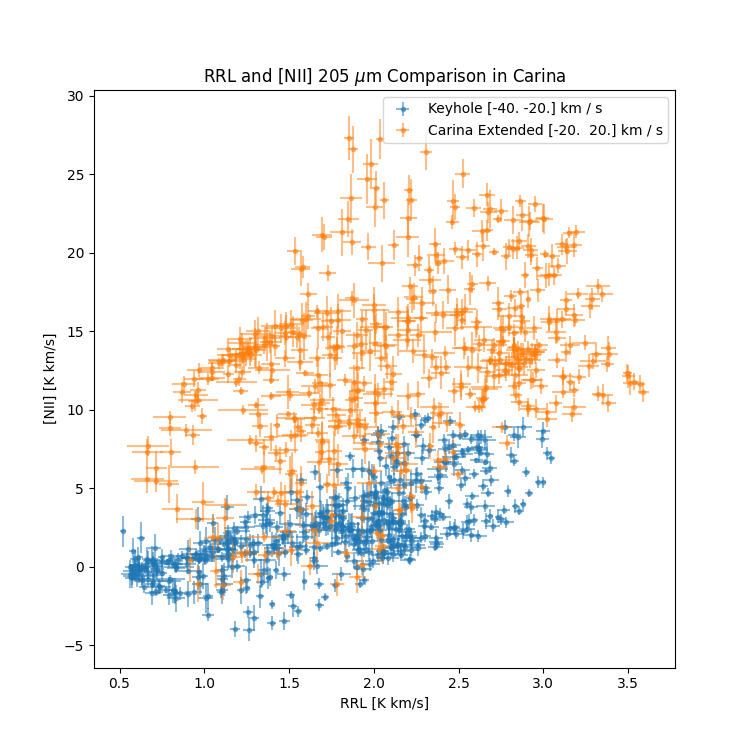
\includegraphics[width=0.6\textwidth]{figs/carina/intensity_scatter.png}
    \caption[Integrated Intensities of {[}NII{]} 205 $\mu$m Line and RRL Data]{
        The integrated intensities of the [NII] 205 $\mu$m line and the RRL data for each pixel in the Carina Nebula.
        The Keyhole Nebula is shown in blue, while the Carina Extended region is shown in orange.
        }
    \label{carina/fig:intensity_scatter}
\end{figure}

Now that we have the integrated intensities of the [NII] 205 $\mu$m line and the RRL data, we can calculate the electron density for each pixel in the map.
Using the Monte Carlo approach, we perform 500 iterations to generate a distribution of electron density values for each pixel.
Many of the pixels in our maps have a low signal-to-noise ratio (SNR), which results in a large uncertainty in the electron density.
In some cases, the root finding algorithm fails to converge, resulting in an undefined value for the electron density.
We omit these values as well as those with an SNR less than 3.
We also omit values whose calculated $n_e$ exceed 1000 as our coverage of the $G_{NLTE}$ coefficients do not extend past that and we would be extrapolating. 
Figure \ref{carina/fig:calculations_keyhole} and \ref{carina/fig:calculations_carina} show the relationship between the density dependent variables of Equation \ref{carina/eq:ratio_final} and the electron density for the Keyhole Nebula and Carina Extended region.
Below that, in Figure \ref{carina/fig:monte_carlo}, we show the the uncertainty of our calculations as a function of the number of samples in our Monte Carlo simulations.
We tested up to 500 samples but, for optimal compute time, we would recommend limiting the value to around 150 as the uncertainty plateaus past that point. 

\begin{figure}
    \centering
    \begin{subfigure}[t]{0.45\textwidth}
        \centering
        
\includegraphics[width=\textwidth]{figs/carina/rhs_keyhole.png}
        \caption{Keyhole Nebula Electron Densities}
        \label{carina/fig:calculations_keyhole}
    \end{subfigure}
    \begin{subfigure}[t]{0.45\textwidth}
        \centering
        
\includegraphics[width=\textwidth]{figs/carina/rhs_carina.png}
        \caption{Carina Extended Electron Densities}
        \label{carina/fig:calculations_carina}
    \end{subfigure}
    \begin{subfigure}[t]{\textwidth}
        \centering
        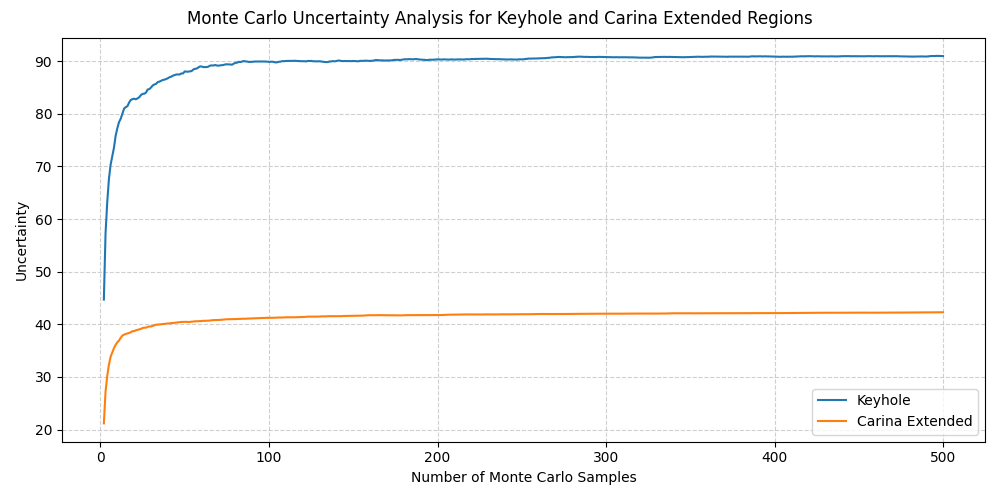
\includegraphics[width=\textwidth]{figs/carina/monte_carlo.png}
        \caption{Measure of Uncertainty in Electron Density Calculations for Both Regions}
        \label{carina/fig:monte_carlo}
    \end{subfigure}
    \caption[Density Dependent Variables for Electron Density Calculations and Monte Carlo Simulation]{
        The density dependent variables of Equation \ref{carina/eq:ratio_final} for the Keyhole Nebula (top left) and Carina Extended region (top right).
        }
    \label{carina/fig:calculations}
\end{figure}

Figures \ref{carina/fig:result_carina} and \ref{carina/fig:result_keyhole} show maps for the [NII] 205 $\mu$m and RRL inputs as well as the calculated electron density for the Carina Extended and the Keyhole Nebula, respectively.
These maps are generated after omitting pixels with an SNR less than 3 and those with an electron density greater than 1000 cm$^{-3}$.
The top panel shows our inputs into the system, the integrated intensity of the [NII] 205 $\mu$m line (left) and the integrated intensity of the RRL data (right).
The [NII] 205 $\mu$m line is shown at the original beam size of the SOFIA data so it can be consistent with the [NII] 122 $\mu$m line below it.

\begin{figure}
    \centering
    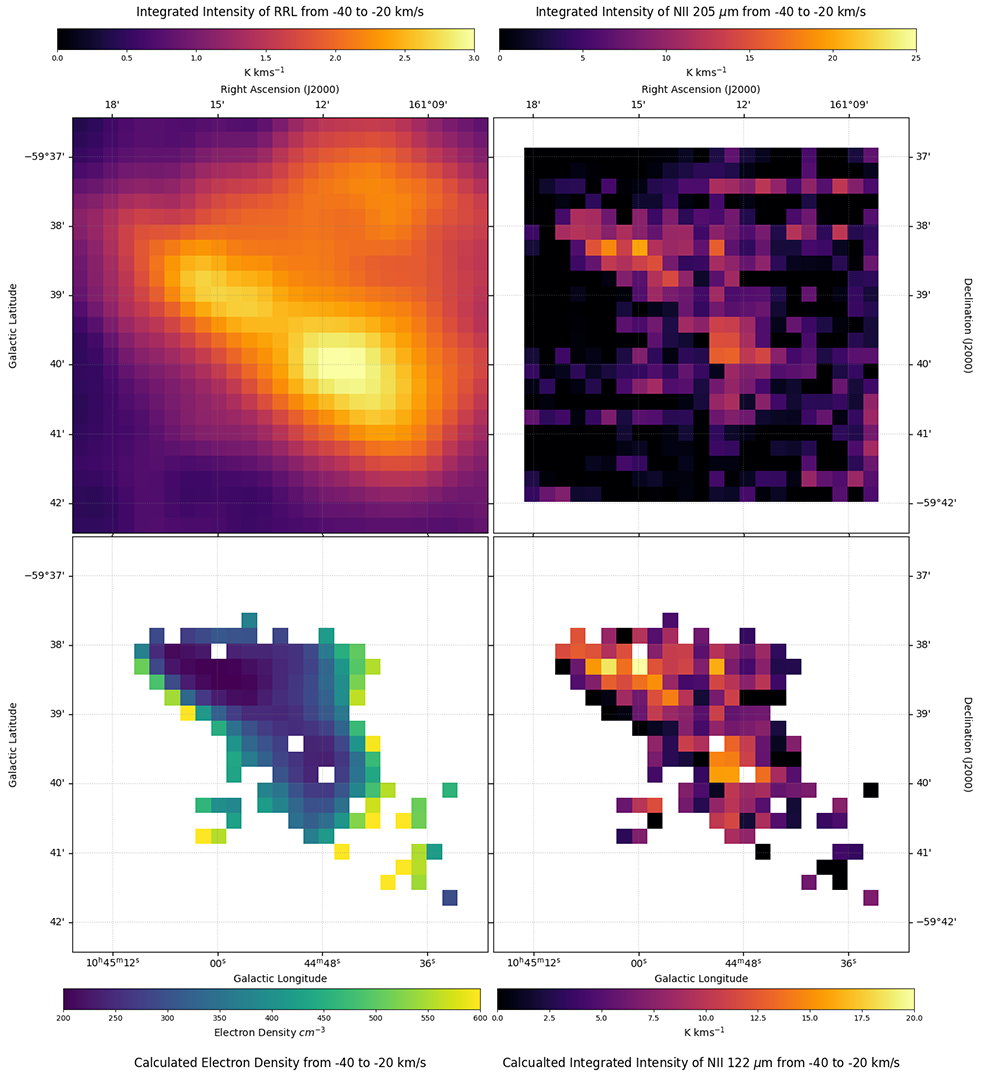
\includegraphics[width=.9\textwidth]{figs/carina/keyhole/keyhole.png}
    \caption[Calculated Electron Density and {[}NII{]} 122 $\mu$m Maps for the Keyhole Nebula]{
        The inputs and outputs of our electron density calculations for the Keyhole Nebula.
        The top left panel shows the integrated intensity of the RRL data, the top right panel shows the integrated intensity of the [NII] 205 $\mu$m line, the bottom left panel shows the calculated electron density, and the bottom right panel shows the estimated integrated intensity of the [NII] 122 $\mu$m line.
        }
    \label{carina/fig:result_keyhole}
\end{figure}

\begin{figure}
    \centering
    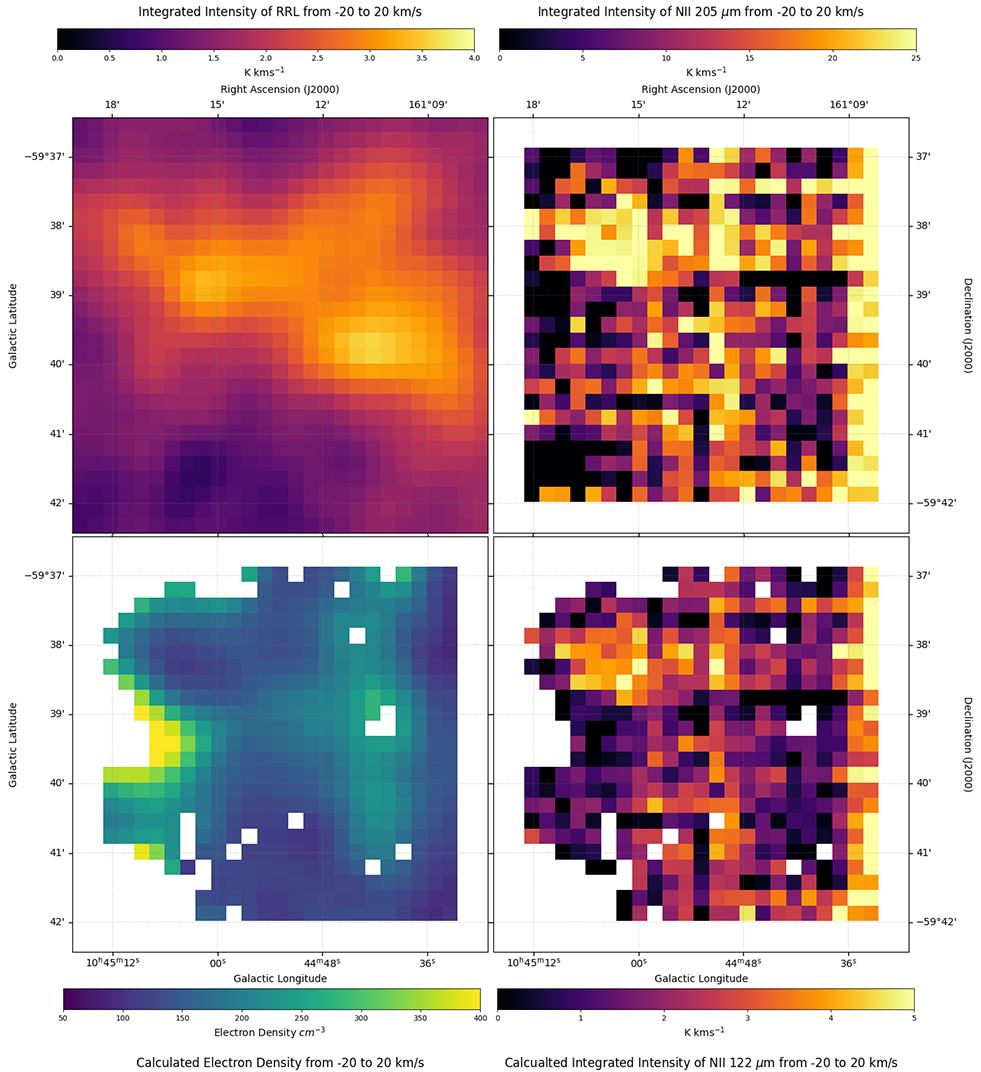
\includegraphics[width=.9\textwidth]{figs/carina/carina/carina.png}
    \caption[Calculated Electron Density and {[}NII{]} 122 $\mu$m Maps for the Extended Carina Nebula]{
        The inputs and outputs of our electron density calculations for the Extended Carina Nebula.
        The top left panel shows the integrated intensity of the RRL data, the top right panel shows the integrated intensity of the [NII] 205 $\mu$m line, the bottom left panel shows the calculated electron density, and the bottom right panel shows the estimated integrated intensity of the [NII] 122 $\mu$m line.
        }
    \label{carina/fig:result_carina}
\end{figure}

\section{Conclusions}
Using the [NII] 205 $\mu$m line and the RRL data, we were able to calculate the electron density in the Carina Nebula.
We found that the Keyhole Nebula has a higher electron density than the Carina Extended region, which is consistent with previous studies \parencite{brooks2000unlocking}.
In comparison to \cite{oberst2011205}, we find that our electron density values are larger than those found in their study.
This makes sense as the spectral resolution of our data is much higher, allowing us to resolve the [NII] 205 $\mu$m line more accurately.
A scatter plot comparing the SPIFI and the SOFIA data is shown in Figure \ref{carina/fig:oberst}, which shows little correlation between the two datasets.
This is likely due to the differences in resolution and sensitivity between the two datasets.

\begin{figure}
    \centering
    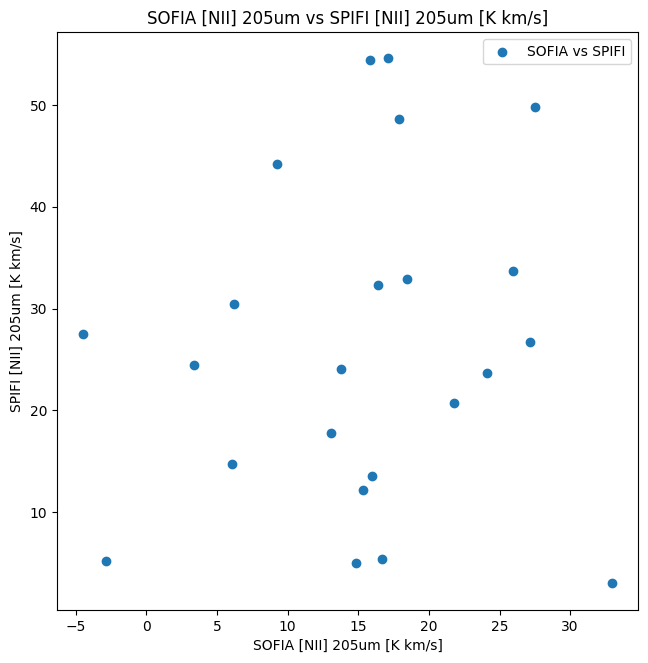
\includegraphics[width=0.6\textwidth]{figs/carina/oberst.png}
    \caption[Scatter Plot of SPIFI and SOFIA {[NII]} 205 $\mu$m Line Intensities]{
        A scatter plot of the SOFIA data (x-axis) and the SPIFI data (y-axis) for the [NII] 205 $\mu$m line.
        Intensities for SOFIA are integrated over the same spectral range as the SPIFI data, centered around the peak of the [NII] 205 $\mu$m line.
        }
    \label{carina/fig:oberst}
\end{figure}

We also estimated the [NII] 122 $\mu$m line intensity using the ratio of the two [NII] lines, which can be used to estimate electron density as well \parencite{goldsmith2015herschel}.
ASTHROS, the Astrophysics Stratospheric Telescope for High Spectral Resolution Observations at Submillimeter Wavelengths, is a proposed mission that will observe the [NII] 122 $\mu$m line and the [NII] 205 $\mu$m line to measure electron density in star-forming regions \parencite{siles2020asthros}.
In the proposal for ASTHROS, the goal is to achieve a signal-to-noise ratio (SNR) of 4 for the [NII] 122 $\mu$m line at a sensitivity of 0.1 K and a SNR of 10 for the [NII] 205 $\mu$m line at a sensitivity of 0.15 K.
We can estimate the signal of our SNR by dividing our integrated intensity by the full width at half maximum (FWHM) of the line.
This can be done at each pixel in our maps to estimate our average signal in Kelvin for both the Keyhole Nebula and the Carina Extended region.
Dividing this signal by the expected sensitivity gives us the SNR for each pixel in our maps, as shown in Figure \ref{carina/fig:snr}.

\begin{figure}
    \centering
    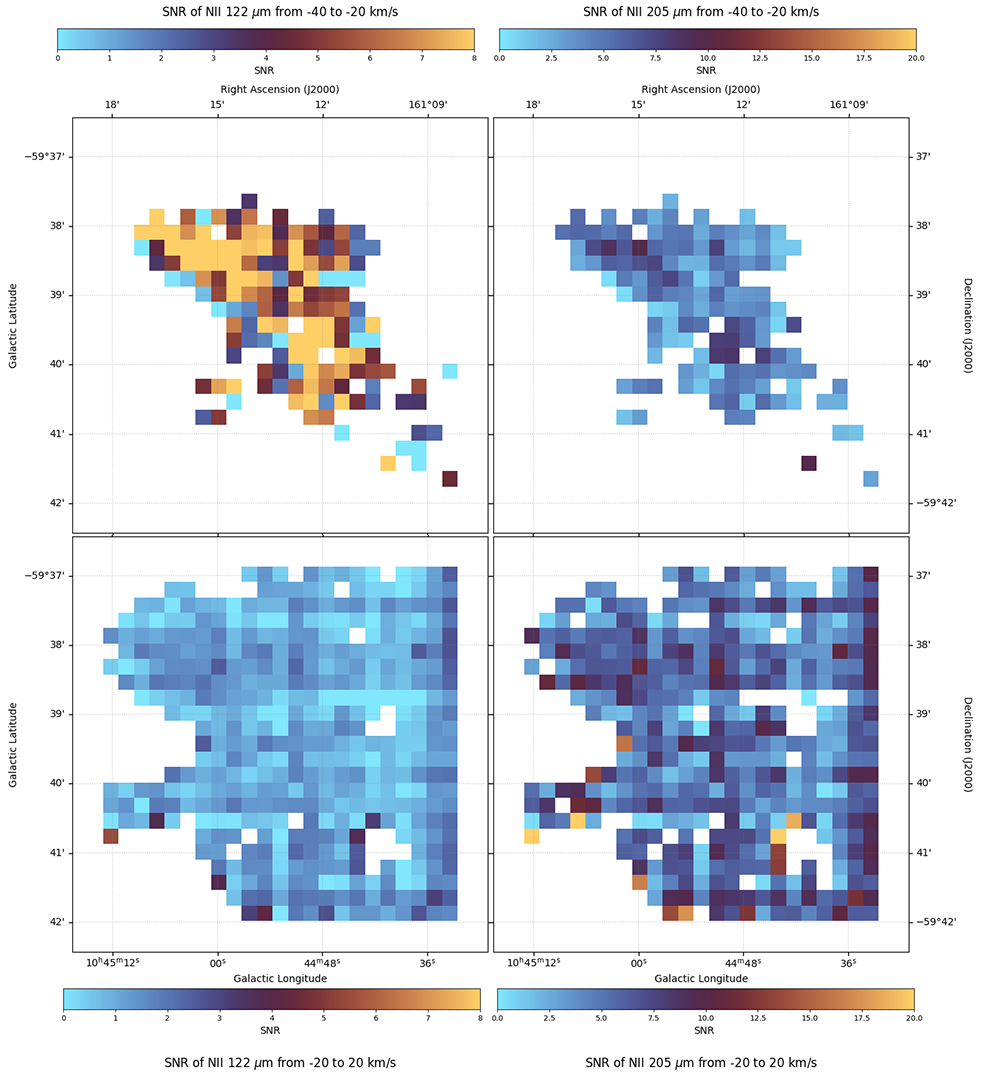
\includegraphics[width=.9\textwidth]{figs/carina/snr.png}
    \caption[SNR of the {[}NII{]} 122 $\mu$m and 205 $\mu$m Lines in Carina Nebula]{
        The signal-to-noise ratio (SNR) of the [NII] 122 $\mu$m line (left) and the [NII] 205 $\mu$m line (right) for both the Keyhole Nebula (top) and the Carina Extended region (bottom).
        The diverging color scale is used to show how close the SNR is to the desired values for ASTHROS.
        For 122 $\mu$m, we want an SNR of 4 at a sensitivity of 0.1 K and for 205 $\mu$m, we want an SNR of 10 at a sensitivity of 0.15 K.
        }
    \label{carina/fig:snr}
\end{figure}

Unfortunately, we find mixed results for the desired SNR in Carina. 
Of the two lines and regions, the Keyhole Nebula's 122 $\mu$m line is the only one that meets the desired SNR of 4, with an average SNR of 5.3.
The 205 $\mu$m line in the Keyhole Nebula has an average SNR of 4.0, which is below the desired SNR of 10.
This makes sense as the electron density is relatively high in the Keyhole Nebula, which results in a higher signal for the [NII] 122 $\mu$m line as shown in Figure \ref{carina/fig:nii_curves}.
The Carina Extended region has an average SNR of 1.1 for the [NII] 122 $\mu$m line and 4.0 for the [NII] 205 $\mu$m line, which is below the desired SNR for both lines.
This is consistent with the lower electron density in the Carina Extended region, which results in a lower signal for the [NII] 122 $\mu$m line.
Overall, these results suggest that ASTHROS needs to improve its sensitivity to observe both lines in the Carina Nebula, especially in the Carina Extended region.
Additional calculations can be done to estimate the amount of integration time necessary to achieve the desired SNR for both lines in the Carina Nebula.
Given that ASTHROS estimated s a sensitivity of 0.1 K for the [NII] 122 $\mu$m line and 0.15 K for the [NII] 205 $\mu$m line, we may be able to improve our SNR by increasing the integration time.